\documentclass[tikz,border=5mm]{standalone}
\usepackage{tikz}
\usetikzlibrary{calc,angles,quotes}

\begin{document}
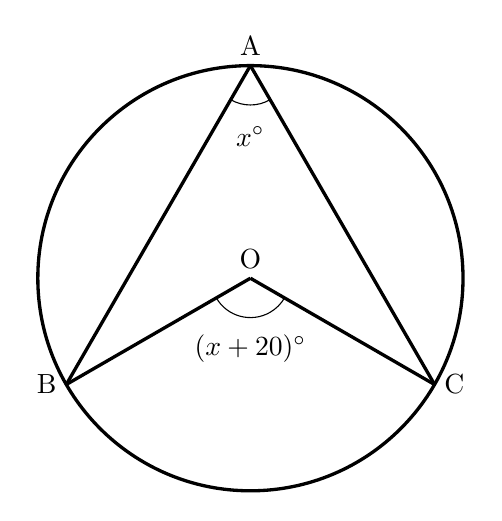
\begin{tikzpicture}[scale=1.8]

% Define the radius
\def\r{1.5}

% Center of circle
\coordinate (O) at (0,0);

% Draw the circle
\draw[very thick] (O) circle (\r);

% Define vertices on the circle
\coordinate (A) at (90:\r);      % Top
\coordinate (B) at (210:\r);     % Bottom left
\coordinate (C) at (330:\r);     % Bottom right

% Draw lines from center O to vertices B and C
\draw[very thick] (O) -- (B);
\draw[very thick] (O) -- (C);

% Draw lines from A to B and C
\draw[very thick] (A) -- (B);
\draw[very thick] (A) -- (C);

% Angle arc at A (x°) - angle BAC inside - LARGER FONT
\pic[draw, angle radius=5mm, angle eccentricity=1.8, "$x^{\circ}$" font=\normalsize] {angle=B--A--C};

% Angle arc at O ((x+20)°) - angle BOC inside
\pic[draw, angle radius=5mm, angle eccentricity=1.8, "$(x+20)^{\circ}$" font=\normalsize] {angle=B--O--C};

% Vertex labels
\node[above] at (A) {A};
\node[left] at (B) {B};
\node[right] at (C) {C};
\node[above] at (O) {O};

\end{tikzpicture}
\end{document}